\documentclass{standalone}

\usepackage{tikz,pgfplots}

\begin{document}
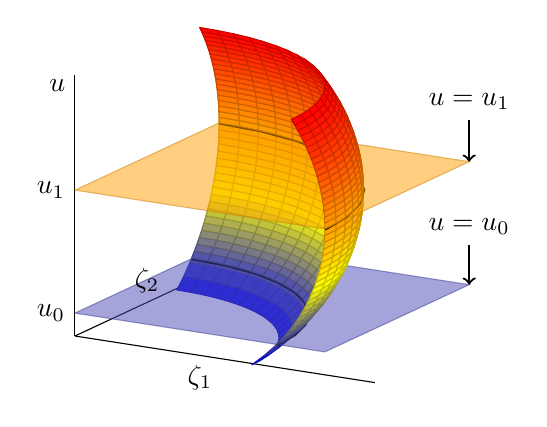
\begin{tikzpicture}
\begin{axis}[clip=false,view={30}{50},
    plot box ratio={1.2}{1.1}{4},
    axis lines*=center,
    xmin = 0,xmax=1.2,
    ymin = 0,ymax=1.1,
    zmin = 0,zmax=1.25,
    grid=minor,
    scale=0.85,
    xtick=\empty,
    ytick=\empty,
    ztick=\empty,
    every axis x label/.style={at={(ticklabel cs:0.9)},anchor= near ticklabel},
    every axis z label/.style={at={(ticklabel cs:0.9)},anchor= near ticklabel}]
%\addplot3[surf, samples=20, domain=pi/2:0,y domain=0:pi/3] ({cos(deg(x)) * sin(deg(y))}, {sin(deg(x)) * sin(deg(y))}, {1-cos(deg(y))});
\addplot3[surf, samples=20, domain=pi/2:0,y domain=pi/4:2*pi/3] ({cos(deg(x)) * sin(deg(y))}, {sin(deg(x)) * sin(deg(y))}, {0.7-cos(deg(y))});
\addplot3[data cs=polar,samples y=0,domain=0:90,samples=10,very thick] (x,0.81,0.11);
\addplot3[data cs=cart,surf,domain=0:1,samples=2, opacity=0.5] {0.11};
\addplot3[surf, samples=20, domain=pi/2:0,y domain=1.2*pi/4:pi/2] ({cos(deg(x)) * sin(deg(y))}, {sin(deg(x)) * sin(deg(y))}, {0.7-cos(deg(y))});
\addplot3[data cs=polar,samples y=0,domain=0:90,samples=10,very thick] (x,1,0.7);
\addplot3[data cs=cart,surf,domain=0:1,samples=2, opacity=0.5] {0.7};
\addplot3[surf, samples=20, domain=pi/2:0,y domain=pi/2:2*pi/3] ({cos(deg(x)) * sin(deg(y))}, {sin(deg(x)) * sin(deg(y))}, {0.7-cos(deg(y))});
%\addplot3[surf, samples=20, domain=pi/2:0,y domain=0:pi/3] ({cos(deg(x)) * sin(deg(y))}, {sin(deg(x)) * sin(deg(y))}, {-cos(deg(y))});
\draw[<-,thick] (axis cs:1,1,0.7) -- (axis cs:1,1,0.9) node[above] {$u=u_1$};
\draw[<-,thick] (axis cs:1,1,0.11) -- (axis cs:1,1,0.3) node[above] {$u=u_0$};
\node[left] at (axis cs:0,0,0.11) {$u_0$};
\node[left] at (axis cs:0,0,0.7) {$u_1$};
\node[above] at (axis cs:0,0.5,0) {$\zeta_2$};
\node[below] at (axis cs:0.5,0,0) {$\zeta_1$};
\node[left] at (axis cs:0,0,1.2) {$u$};
\end{axis} 
\end{tikzpicture}
\end{document}
